.
However, they contribute much less to the public transfer system during the entire life, and especially during their working life -> it is explained by lower labour income at each age for immigrants (mettre graphique de revenus du travail?) and thus less taxes on income (Direct taxes from persons from immigrants accounts only for 22.7\% of direct taxes while they represent 25.6\% of the population) and they consume therefore less than natives (22.9\% of Taxes on products and imports are made by immigrants), as demonstrated in table 1.

On average between 1997 abnd 2015, immigrants contribute for about \$\DTLfetch{statex}{sKey}{AvePmtImmigrantOutflows}{sVal} per year while receiving about \$\DTLfetch{statex}{sKey}{AvePmtImmigrantInflows}{sVal}\$ per year in average betwen 1997 and 2015. native on the other hand contributed \$\DTLfetch{statex}{sKey}{AveCanadianBornOutflows}{sVal} but received \$\DTLfetch{statex}{sKey}{AveCanadianBornInflows}{sVal}.

If immigration is costly to public finances, the opposite appear to be true for corporate finances which finance little to none of the cost but are the main beneficiary of its output through the labour market.




However, \citet{Hermansen:2017ht} found that older age at arrival has a negative and long-term impact on educational attainment and labour market success.

\vspace{0.7em}\par
The so called socio economic status that play such a determinant role in population research and other social sciences, are the embodiment of a self perpetuating inequality system. They are endogenous compoments to, and the main causes of, differences in society and human behavoirs. Social classification is the requirement for economic inequality while the latter back fuel the former in a vicious cycle. Immigration just happen to be a mean, or rahter the mordern time mean for entry into the lower classes, just like slavery and other forms of mass subjugation before it. But the social system that call them forth has exited since the dawn of human civilization. Is change possible? Superfial changes are possible and have happened from time to time. But even such changes have happened too late, after and at the cost of, much revolution and distress. Real changes are impossible unless our collective consciousness reach a point that allow humanity to overcome its fears. When and wether this possibility will be realized are questions that we leave to better equiped mind. The world and Canada would need agile and well-rounded(CHANGE) thinkers who can assess the bulding block of society and engage the changes required for the kind of the society we leave to next generations. The responsibility rests upon the shoulders of the accademic world to guide policatical decision.





Cette contradiction apparente dans les études est liée, entre autres, à l'utilisation de différents sous-ensembles de la population immigrante \citep{Grubel:2012wo} et aux différents coûts et contributions considérés \citep{dAlbis:2019de}. Une meilleure évaluation de l'impact fiscal de l'immigration devra donc considérer, pour plusieurs générations d'Immigrants, les contributions(taxes et impôts) d'une part et les transferts (familiaux et publics) d'autre part, et ceci en comparaison avec les natifs. L'approche NTA (National Transfer Account) proposée par \citet{Mason:2011wc} semble prometteuse pour répondre à ces défis, mais à notre connaissance aucune étude au Canada n'en a fait usage dans ce contexte.

tant les débats sur le role de l'Immigrants dans un contexe de vieillissement démographique continue, tant les gouvernements sucessives ont jugé utile




permis d'établire un consenus sur le role de l'immigration, ni proposer des sources alternatives et significative de main-d’œuvre pour palier aux effets du vieillissement population.



 Au Canada, entre  les années 1990 et 2016, un nombre relativement élevé d’Immigrants ont été reçus, avec une moyenne d’environ 235 000 par année \citep{StatistiqueCanada:2016ud}. Alors que certains justifient ces niveaux élevés d’immigration par des raisons économiques \citep{Christine:2015tu,Newton:1981jy}, d’autres sont plutôt d’avis que les objectifs économiques ne devraient pas constituer la raison première de la politique d’immigration et que, dans un avenir immédiat, d’autres politiques mieux adaptées permettraient d’atteindre ces objectifs \citep{Gingras:2000dk,Green:1999ko,McDaniel:2013kf,Wong:2015uz}.



\textbf{Limites}
comparing immig vs native remove the effect of macro eco condition which are assume to affect immig and native similary.


Because the canadian population is in it sources built by immigrant, the percent of immigrant at a higer is much greater than at younger age. because the more we go back in time, the most like are people born outside canada.




\textbf{Who is an immigrant?}
Static estimates of fiscal impact designate a certain group of people as immigrants and then calculate the amount of tax they pay and how much government expenditure they absorb. Deciding who is an immigrant for this purpose is not a simple matter. On a strict interpretation, an immigrant is any resident who was born abroad. Such a definition would normally overstate the fiscal contribution of immigrants because it would exclude government expenditure on their locally born children. In practice no study uses such a narrow definition. For example, Smith and Edmonston (1997, ch. 6) estimate the fiscal contribution of all US households with an immigrant head. This includes children and other dependants who are resident in the household. It also includes the native spouse of an immigrant head of household, but excludes the immigrant spouse of a native head of household. In their study of UK immigration, Gott and Johnson (2002) take a more individualist approach and classify as an immigrant anyone who is foreign-born, or who is a child under 16 and has two parents who are foreign-born or a lone parent who is foreign-born. They classify as natives all children aged 16+ who were born in the UK and also children under 16 who were born in the UK and have at least one native parent. There are arguments for and against the various definitions, and the choice of which definition to use is often heavily influenced by the information that is available. \citep{Rowthorn:kk}



\citep{Bratsberg:2014cl}
p.2: Dustmann and Frattini (2014) present evidence from the UK that the direct fiscal contribution differs importantly by immigrant origin. With considerable variation in the composition of migrant flows across time and space (Bauer et al., 2000), the overall fiscal impacts will vary across destination countries depending on the relative skills and origin mix of the immigrant population -- Highlighted Sep 15, 2019

p.27: In the longer term, the fiscal impacts of immigration will hinge on the human capital accumulation and labour market outcomes of their descendants. Fertility differences between immigrants and natives also form a key factor in the dynamic analysis of fiscal consequences of immigration, as higher fertility in the immigrant population will alter the composition of age groups with negative and positive fiscal balances (Preston, 2014). The rate of immigrant–native convergence in fertility is of interest in its own right as it signals the degree of immigrant integration and assimilation in general -- Highlighted Sep 15, 2019

p.35: The broader fiscal analysis has to include contributions and expenditures over the complete lifecycle, taking into account that tax payers do not have to pay the costs of child care and education before immigrants arrive and that some immigrants will spend the last – and most cost intensive in terms of health care – years of their life in their country of origin -- Highlighted Sep 15, 2019

However, there are other labour market effects that may be beneficial to Canadian-born workers, investors, and landholders. For example, the lower average wage of immigrants provides a cheap labour input for firms, which in turn, generates higher profits. Indeed, Dustmann et al. (2008) finds that immigrant workers raise the incomes of most native-born workers. Additionally, immigrants increase the production and variety of goods and services in the economy. This can result in increased innovation and specialization. immigrants also provide a boost to international trade. \citep{Javdani:2013gu}


Population aging has becomme the driver of many heated debates and one of the fierce is the role of immigration not only as source of additional labour supply but also as one of the possible solutions to securing income for the public purse \citep{Hansen:2017uz}.


  A lot has been written about the effect of immigration on host countries. Studies cover many aspects, including, the labour market \citep{Borjas:2003cr,Dustmann:2016by}, the wages \citep{Dustmann:2013hk,Eberhard:2012te},  school performance \citep{Brunello:2013cy}, crime \citep{Chalfin:2015fb}, the overall welfare in the economy \citep{Ileri:2019hf,Akin:gh,Dungan:2013jp,Fougere:2011ht}, inovation \citep{Hunt:2008fn,Partridge:2008up}



  While the impact of immigration on various aspect of the labour market has been extensively researched, the fiscal consequences, an even more important concerns by public opinion \citep{Dustmann:2014dr}, for receiving countries are less obvious \citep{Preston:2014uw}.

  Public policies on immigration are to no small extent affected by public opinion about immigrant which in turn is characterised by some form of hostility toward immigrants on the premices that immigrats do not pay their fair share to the tax system or receive more than their contribute to the welfare system\citep{Dustmann:2007fl}. For example the 2008 European Social Survey reveal that, 44\% of European citizens responded that immigrants receive more than they contribute, with only 15\% believing that they receive less \citep{Dustmann:2014dr}.

  The overall effect vary from negative to positive depending on the timeframe covered and th composition of the immigration population including their countries of origin\citep{Clarke:2013dh,Hansen:2017uz}, skills and occupations; past and current host countries immigration and welfare systems; as well as the analytical methododology


  \citep{Hansen:2017uz} found that that immigrants from Western countries to Denmark have a positive fiscal impact, while immigrants from non-Western countries have a large negative one. Inded, the country of origin not only affect labour market outcome particularly in average earnings \citep{Clarke:2013dh} but also their contribution to the public purse as lower income means lower taxes. This is particulary the case in Canada, where labour market outcome(earning and unemployment of immigrant) has worsen during the last decade.





  The simulations from \citep{Dungan:2013jp} indicate that additional immigration is likely to have a positive impact on the Canadian economy including government expenditures, taxes and especially net government balances, with essentially no impact on unemployment.

  \citep{Ileri:2019hf} found that skilled immigration lower wages inequality and contributes positively to the overall welfare in the economy





  \citep{Akin:gh} found that a prohibition on immigration reduces welfare for the natives, whereas a policy that allows an annual inflow equal to 0.4 percent of the population increases welfare for all agents. Although immigration reduces wages, it raises the rental rate of capital and the number of workers per retiree, allowing for higher pension benefits and a lower consumption tax rate.






    % note immig begin------------------------
  \footnotetext{\label{note:immig} Sources: Statistics Canada, Census of Population, 1871 to 2006, 2016; National Household Survey, 2011; Immigration and Diversity: Population Projections for Canada and its Regions, 2011 to 2036 (reference scenario).. Voir \url{https://www.statcan.gc.ca/eng/dai/btd/othervisuals/other006}}
  % note immig fin----

  This study departed from the above by focusing on the canadian perpective which differ from US and Europe at least in the following ways that could mitigate the effect.

  Canada stand out of the OECD countries with one of the most selective immigracy system, a relatively large immigrant population(\hyperref[note:immig]{21\%\footnotemark}) and its vaste amount of data.


  For Canada, recent studies has not addressed the question of fiscal impact and much older studies has been not reached any consensus.



  Our also differ the these by introduction the NTA methododology which make less assumption about futures immigration characteriscs and government revenu and spending






  Canada also differ from US and European countries for it relative immigration population share(reference and percentage), It is therefore important to investigate whether immigration impact on Canada welfare system diverge or converge to the conclusions from the US and European.


  This paper differ from and complemente the current litterature three important dimension.
  First it take advantage of a much longer time framework and a larger data source. Almost 4 decades of data covering, labour, income, taxe files et census data has been used

  second, it integrate an intergenerational approach into the cost/benefits accounting



  This study is also the first of its kind to integrate immigration status into the NTA framework.

  Despite the great interest

  Result varies from countries to countries as each countries has different immigrants intake and integration programs.

  Immigration is coslty to many member of the host country. That's the clear message echoed in borjas's latest book: Immigration Economics \citep{Card:2016ku}, the 30 years summary of the author's work in the field of immigration. And yet, immigrant intake has been increasing in most developed country over the last last decades and will continue to do so in the decades to come. Obvously,  \citep{Borjas:2014hr} present one side of the story of the which another side is that skilled migrants make a large fiscal contribution, whereas unskilled migrants may be net contributors if they eventually depart and make few claims on government expenditure while in the country \citep{Rowthorn:2008kk}.

  Most of what is known about the fiscal impact of immigration comes from studies on European countries and the United States. Very little is known about the net contribution of immigrants to the public finances in Canada, even though, it has some of the most structured immigration policies and programs

  With its particular immigration system and large amount of realiable data on immigration participation, Canada has substancial contribution to the fiscal aspect of the immigration debate.

  With this opposing results in empriral findings in europe et USA, the Canadian case would help strenthen one or other side.

  Increasing the retirement age has been propose  to alleviate the pressure on CPP and QPP brought about by population aging as an alternative to immigration \citep{Hering.Klassen.2010}

  \citep{Hering.Klassen.2010} have found that increasing would significantly improve the fiscal sustainability of the CPP and largely solve the financing problems of the QPP

  While some see immigrants as a fiscal drain, othe perceive in as potential solution to the fiscal pressures from popolationg aging \citep{RePEc:nbr:nberch:10849} which will worsen during during the comming decades.

  some has suggested that attention should be paid to the composition rather than the level of the immigrant population \citep{RePEc:nbr:nberch:10849}. But in the canadian context, skills and education attainement recognized constitue a bariere for swith in paradime. Therefor, even with this long years experience in immigrations Canada still has a long way to go in taking full advantage of the potential of its immigrants.








  immigrants differ from natives in demographic type, in skills and in customs and consequently pay different taxes and impose differently on public services \citep{Preston:2014uw}

  There is a popular belief that immigrant are firscal burden. Belief that is not is usually not supported by empirical result.

  \citep{Grubel:2012wo} found that in the fiscal year 2005/2006 the average immigrant costed \$6,051,  While \citep{Javdani:2013gu} reported about \$500 and even this negative impact result from the degradation in the composition and income attainement of immigrant over time. Indeed, using data from the 1981 census, \citep{Akbari:1989fh} a positive net fiscal transfer of \$500
  The auhtor warn that given immigrant are paid less compaire to native same similar socido demographic status, such result should not be use as the base for public polici

  in a later publication, \citep{grady2015immigration} wrote ... the number of annual immigrants needs to be reduced to bring about a substantial reduction in total fiscal burden imposed by new immigrants on Canadian taxpayers.

  Over the same period (2005/2006) \citep{Javdani:2013gu}




their calculations indicate that definition of the study population is critical to the outcome. If limited to immigrants themselves, the overall fiscal impact is \$1,400 (taxes paid less costs generated) per immigrant. If limited to immigrants plus their U.S.-born children under the age of 20, corresponding to the immigrant household formulation, the average fiscal impact is about -\$600 per immigrant (or -\$400 per immigrant and young child). If extended to all descendants of living immigrants, the average fiscal impact is \$1,000 expressed per immigrant, or \$600 expressed per immigrant and descendants.






  Taking the complete life cylce into account, most immigrants arrive in the host country during a period of the lifecycle where production surpasse greatly consumption. Therefore, immigration represent a saving to tax payer as they do not have to pay the costs of child care and education before immigrants arrive \citep{Bratsberg:2014cl}. For example, \citet{Dustmann:2014dr} found that  between 1995 and 2011 European and non-European immigrants endowed the UK labour market with human capital that would have cost £14 and £35 billion respectively, if it were produced through the British education system. Moreover, some will return to their country of origin to spend the last and most cost intensive in health care \citep{Bratsberg:2014cl}


  constracting to this public view, are the finding from \citep{Dustmann:2014dr} that provide strong evidence that immigrants expecially recent ones, has made substancial contribution to public finances by contributing far more in taxes than they have received in benefits.

  But this varies from country to country in the developed world.
  Using a similar approach, \citep{Chojnicki:2011vu} found that even though the long term effect of immigration on public finances is slightly positive, the life cycle average of immigration net contribution is negative for the year 2005 in France.



  Fiscal effet of immigration varies on the methododology on one hand and the immigrant population on the other hand. \citep{Chojnicki:2011vu,Lee:1998fs}

  Also as any policy effect unfold in time, the life cycle approach make much sense as it allow to integrate not changing characteriscs of the immigration over time but also the effect of long term policy.

  A problem with longitudinal studies is that they are based on forecasts of future government expenditures, the economic impact of immigrants and their descendants, and future tax rates—three variables that are constantly in flux and ex ante unknowable.


  Because fiscal impacts are distributed over the lifetimes of the immigrants and their descendants, ignoring any of these sub group will inivitably result in biaised estimations.




  This paper doesn't concerne with weither, how much and to what extend future immigration can mitigate the increased fiscal stresses expected from changing demographic structure. It will however provide answer to questions on wether immigrant paie their fair share in reference to native canadian.

  Studies that evalutate fiscal impact of immigration without compairing with native may provide some insight of the net cost of immigration but still unaable to support

  As \citep{Fehr:2003gq} stated, even doubling the number of immigrants, and extreme mesure by most policy standards, will little to mitigate the upcomming finacial pressure in developed countries.

  This contrast with the result from \citep{Storesletten:2000cn} who found that selective immigration policies, involving an increased inflow of working-age high and medium-skilled immigrants, can remove the need for future fiscal reform. For instance, an intake annual intake of of 1.6 million (an increase from 0.44 to 0.62 of the population) immigrants is equivalent to increasing taxe revenu by 4.4 percentage points in the US.


  In the main there are two dimenssion that are most important. The time scope, that is weither the study is dynamic or static, and the scope of the immigrant population, that is the number of immigrants generation included.

  These two elements intertwined and one can't really consider the first without touching the other.



  Using various scope of the immigration population, \citep{Lee:1998fs}  found that, the overall fiscal impact (taxes paid less costs generated) is in average, \$1,400 if only first generation immigrants are included, -\$400 if second generation is included, and  \$600 if extended to all descendants of living immigrants.

  Most recents studies focused on some subset of the immigrant population.

  Also as any policy effect unfold in time, the life cycle approach make much sense as it allow to integrate not changing characteriscs of the immigration over time but also the effect of long term policy.





  If hostile opinion in the the public toward immigrants can be attributed to the perception that  that they receive more out of public finances than they contribute to it, then, research ought to produce empirical evidence that clarify theses position, Yet, very little evidence is available(at least to the public) on how much immigrate contribute and benefit from public finance.

  Because fiscal impacts are distributed over the lifetimes of the immigrants and their descendants, ignoring any of these sub group will inivitably result in biaised estimations.


  This paper doesn't concerne with weither, how much and to what extend future immigration can mitigate the increased fiscal stresses expected from changing demographic structure. It will however provide answer to questions on wether immigrant paie their fair share in reference to native canadian.




  \citep{Lee:1998fs} was one of the firsts  to take into account both the various definitions and the lifecycl


  The debats now

populating aging may bring labour shortage and presure on finance
Immigratin may help
Because debat is going on
Take position on weither to encourage or restrict immigration
Does immigrant cost more less to the state than native
Fiscal impact of immigration


p.168: La conse?quence a? long terme de l’immigration sera l’apparition de socie?te?s multiculturelles, qui renouvellera les concepts de citoyennete? et d’ tat. -- pichée


In another words while previous immigration policy would be to preventing foreign invasion of the labour market and the degradation of native employment opportunity, recent policy have moved to attract and retain most competitive skilled worker.



It's fundamentally impossible for the govenement to manage economic immigrants since economic managmeent of are not primaly its purpose. This legal justification is not the most important however. Business demande for labour are consistently changing and yet reflect the medium to long term strategy. and only these business can know best enough to select and retain what profile is best.

govenement must have play an arbitration role setting the guideline and making sure they are respected. Among other, the most important is that of equal for immigrant and native, all else equal. This forme of immigration already existe but is very limited. In other word, LIMA should be applied to all economic immigration.



The main conclusion from Borjas's work is that immigration is only susceptible to affect labour opportunity of low-skilled native\citep{Piche:2013ir}

the results from \citet{Fusaro:2018wi} indicate a positive impact on high-educated natives and a strong negative one on low-educated



From a capistalim perspective, they will be a demand for immigrants as slong as it tanslate into more corporate profit. Therefor calls form immigrant from business owner in the name of labour shortage should be given less weight when deciding on immigration policy. Instead public policy should be focussed first and formost emprique research. These may disagre in on a number of matter mostly theoritical, but would converge on important issue that can be used for public policy.

For immigrant to receive slighly more in transfer can be attribute to their higher level of unemployment and other basic difference. However, the difference in outflow transfer which is mostly attribute to difference in revenu is too large to be ingored.

Should gouvernment fail to understand or resolve these differences, the capistalim nature of these difference will push the limit, leading to social conflict.





@Julien
as confirmer pour les o a 5 ans
We assume that all immigrants and natives are enrolled at school before 15 years old.

Avec ces resutlat il serait peut revoir les données et nos hyphothèse pour etre sur que ces derniers n'en sont pas les origines. Si tout va bien à ces niveau on devrait pouvoir retrouver dans l'actualité des ces periodes les raisons qui ont provoquer ces changements qui apparement ne retablissent pas.

Comment expliquer la forme irregulier du graphic 1:B, et les valeur de 2015 par rapport a la figure 2:A

Autre transfers: quelles les aggregats utiliser pour cette section


The expected cost estimated has no much value in their but can be used to access the relative value of immigration to the Canadian economie, and may help toward policies alternative to immigrationà


Immigrants have higher average cost because the average immigrant is aged between x and x, a group age within which consumption largerly surpass production expecially for immigrant as they have to reset their carrier after arivale.





The question of if immigration is irrelevant in the canadian context for the following raisons,
Everyone in Canada is immigrant at some time in history, and the further we go back in time the greater the is the relative proportion of immigrant in the population.



Today's native are yesterday immigrants. From the 2016 cenus for example (Catalogue number :98-400-X2016236). While first generation immigrant represent 23.85\% include second generation increase the immigrant population share to 41.56\%.

We should be concerning with increasing wellbing for all



\subsection{Exploring APC patterns}\label{sec:apc}
  \autoref{fig:surfAll} analyses the age-period-cohort patterns  in transfer differencial on a Lexis plot. The differencial is obtained by substracting the value(of contribution for example) for native from that of immigrant and then rescaling to fit the interval -1 to 1. In the case of contribution, negative one denated by the yellow color means that immigrants contribute in taxes more than native. Positive one on the other hand means that natives make more contribution in taxes than immigrants.

  (very favorable) to 1 (very devaforable) to denote the the extent to which an immigrant cost more or less than a native. The curves on the surface are the APC curvatures that attempt to detect any age, period or cohort effect that may be prevaling.

\begin{figure}[H]%
  \caption{Lexis surface for Transfer differencial(Immigrant-native) in Contribution, Cost and Net Cost between 1997 and 2015}
  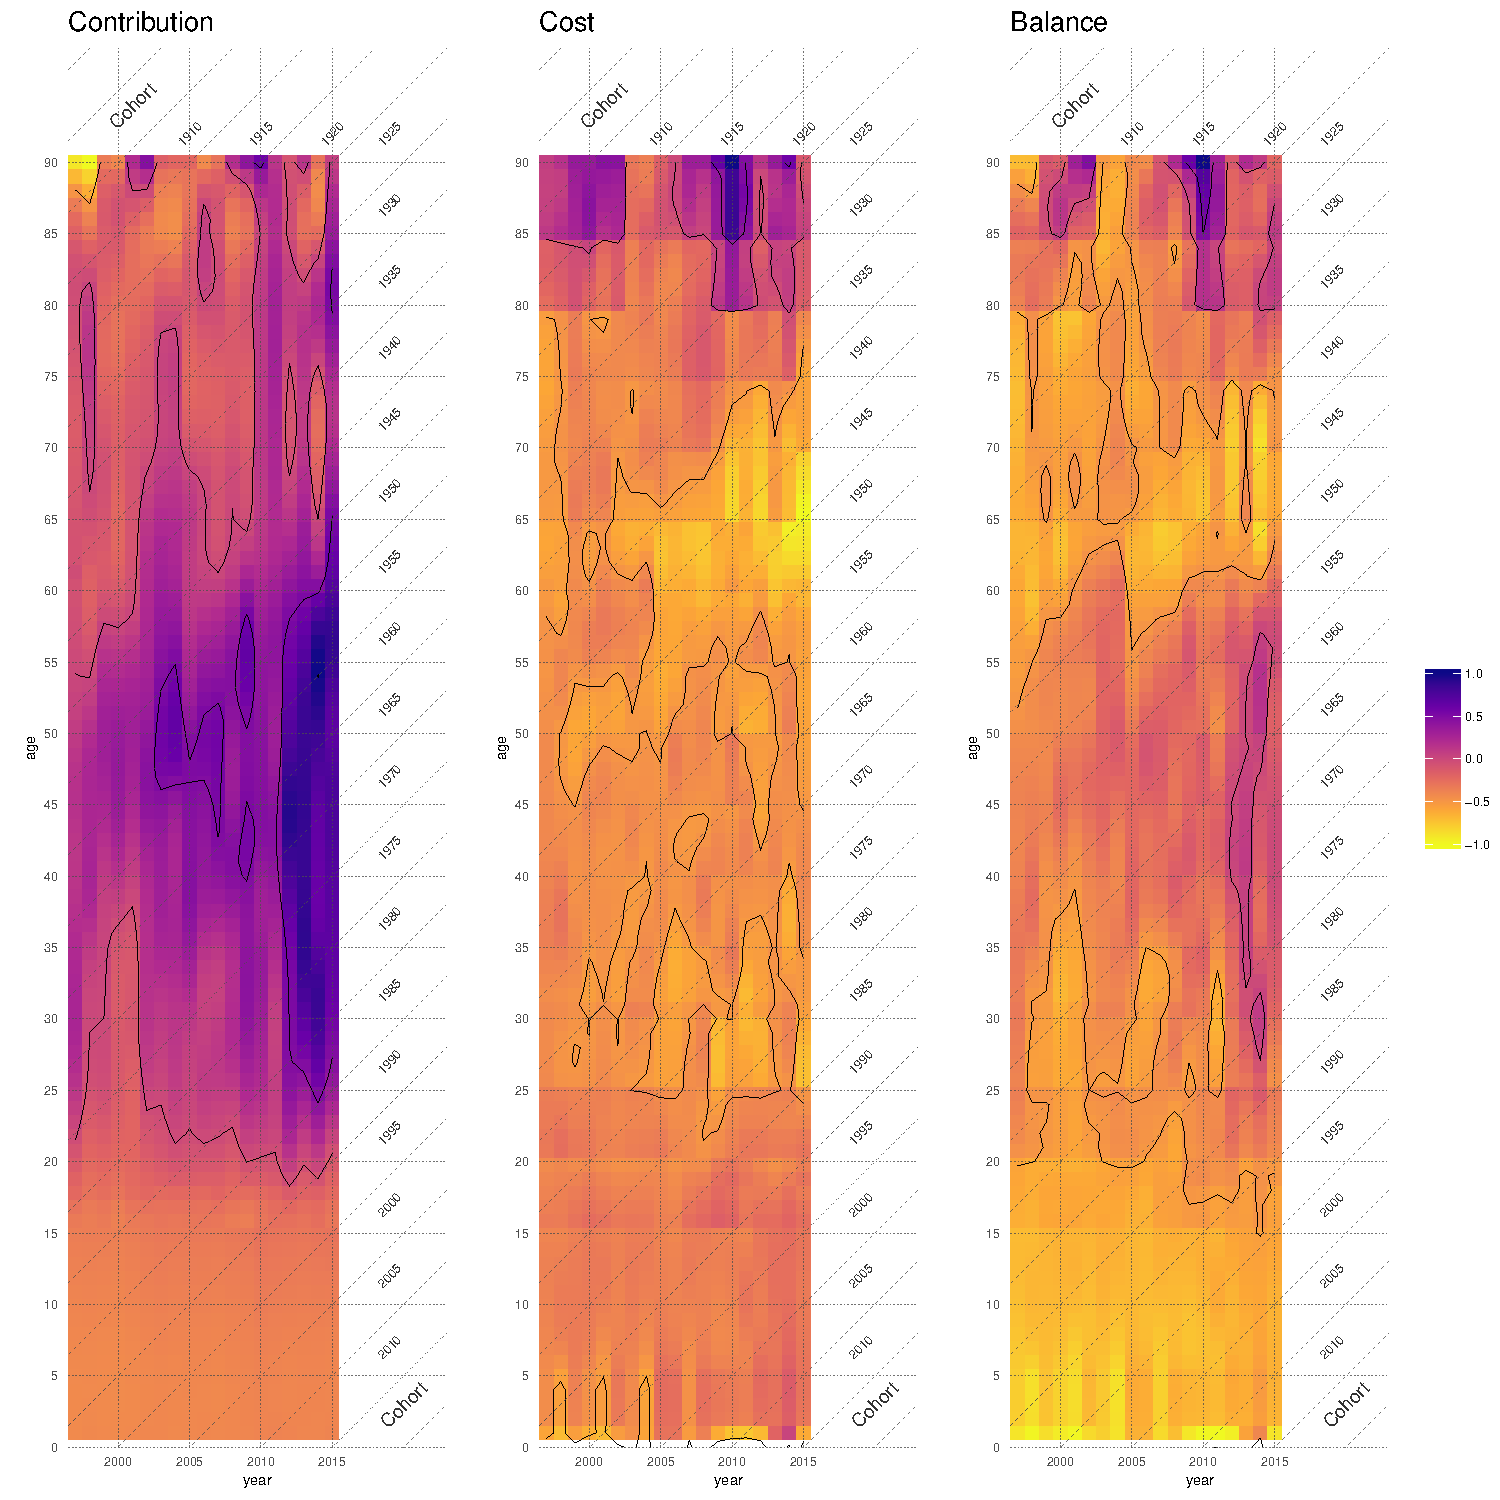
\includegraphics[width=1\textwidth]{./res/surfAll.pdf}%
  \label{fig:surfAll}%
\end{figure}%



  \autoref{fig:surfAll} suggest that immigrant tend to receive more transfer and to contribute less than native. However, transfer differencial between immigrant and native is more pronounced and most defavorable for immigrant in terms of contrubution.